%\documentclass{article}
\documentclass[conference]{IEEEtran}

\usepackage{url}
\usepackage{balance}
\usepackage{amsmath,graphicx}
\usepackage{amsmath}
\usepackage[linesnumbered,ruled]{algorithm2e}
\usepackage{float}
\usepackage{stfloats}
\usepackage{caption}
\usepackage{amsmath}
\usepackage{verbatim}

% Example definitions.

% --------------------
\def\x{{\mathbf x}}
\def\L{{\cal L}}

% Title.

% ------
\title{A Game Prediction Algorithm for Dota}
\author{
    \begin{tabular}{ccc}
    RunZhou Cao & Xiaohu Zhao & Fang Zhou
    \end{tabular}  \\
%    \hspace{1pc}~\\
    \begin{tabular}{c}
    Ohio State University\\
    \end{tabular}
}\begin{document}
%\ninept
%
\maketitle
%
\begin{abstract}
Dota is one of the most popular eSports because of its high entertainment.
There are only few machine learning algorithms for Dota game prediction.
The exisiting research faces several problems so that the results cannot
be reliable.

In this paper, we design a new algorithm for Dota game prediciton.  
First, we design a comprehensive feature vector used in the machine learning algorithms.
Second, we try different machine learning algorithms to choose the best one.
Last but not least, the data scale in our experiments is so large that the results can be reliable.
The results show our algorithm is both effective and efficient.

\end{abstract}

\section{Introduction}

ESports, also known as electronic sports, has become an official sport since the 21st century.
The new technologies applied in the eSports are attractive to the young and old.
The 3D graphic display, vivid sound effect, immersive experience, and the interesting operations make eSports more and more popular.
According to a report~\cite{esports}, In 2013, it was estimated that approximately 71.5 million people worldwide watched eSports.

Since eSports games are increasingly popular, the prediction of eSports game result has become increasingly significant.
The estimation of game results can be used to train the professional players at ordinary times and modify the gamer’s tactic for the upcoming game.
This estimation can also be used for media.
In addition, the predictions of the game results can improve the entertainment for fans.

Therefore, we decide to design and implement a prediction system based on machine learning technology for eSports games.
In this paper, we focus on the one of the most popular eSports games is Dota.
Dota is the short name for Defense of the Ancients.
Dota~\cite{dotablog} is a free-to-play multiplayer online battle arena video game.
Two five-player teams compete in the playing field, where each player chooses one from a total of 111 heroes to play.
Millions of game players take part in Dota every day.
With the highly-speed development of eSports, abundant and grand eSports competitions are organized globally every month, season, and year.
Prize pool of millions of dollars is often provided by some competitions.

Prior research 
Conley et al.~\cite{conley2013does} did a research on which machine learning method is the best for data game results.
However, they only focus on two machine learning approaches, linear regression and k-nearest neighbour(kNN).
Kalyannaraman~\cite{kau2013win} did an augmented algorithm on traditional linear regression considering pair relationships of heroes.
However, he did not consider all the relationship between heroes, like the restraint relationship between heroes.
What's more, these two research did not test on large scale of data, which means not so reliable on their results.
Drachen et al. ~\cite{drachen2014skill} try to predict the temporal and spatial of players in the game based on the hero skills.
But the objective is different from ours. 

Our goal is to predict the results of Dota Game.
It means, given the specific two groups of heroes, we can give back the users the predicted outcome of the game.
In this paper, the contributions include:

\begin{itemize}
\item We are the first one to consider the restraint relationship of heroes into the prediciton of Dota game result. 
\item We are the first one to introduce the game lasting time as a feature vector in the prediction. 
\item We abstract the Dota game prediction problem and applied different machine learning approaches.
\item Through tuning the parameters in the machine learning approaches, we compare the performance among different algorithms. We also conclude the results and analyze the results.
\end{itemize}

The rest of the paper proceeds as follows.
Section 2 introduces Dota and mainstream machine learning algorithms we try in this paper.
Section 3 gives a brief introduction about the abstract of the problem and the goal.
Then in the section 4, we talk about the design of our machine learning algorithms; also a detailed description of Decision Tree is given.
In the section 5, we will describe our data sets, training and testing methods, evaluation metrics and results.
Section 6 introduces some related papers.
In the final section, we will analyze the results of the prediction.

\section{Background}
In this section, we first introduce Dota game.
Then, we continue to introduce the meachine learning algorithms we want to test in this paper. 

\subsection{Dota}
In each dota game, there are two teams against each other, radiant and dire.
Each team consists of five players.
Before starting the game, the players one by one choose one hero from the hero pool, which includes 111 heroes in total.
Different heroes has different skills and play different roles in the team.
The buildings in the game have health points.
The final objective of Dota is to destory the enemy base, which means they want to make the enemy base's health points become 0. 

Even though different heroes have different skills, we can always classify the heroes into four categories: Carry, Support, Ganker, and Initiator.

\begin{itemize}
\item \textbf{Carry:}
These heroes play the core role in a team.
They are the main attack output of a team.
Usually, there are only one carry in a team.
But sometimes, maybe another carry is picked up in case that the main carry cannot develop very well.
However, at first, these heroes are not good at battle so they need some time to level up.
They usually take over the game in the group battle at the end of a game.
In most cases, all the behaviors of other heores in a team serve for the carry heroes.
For example, other heroes always protect the carry's life and sometimes they choose to die instead of the carry hero.
\item \textbf{Support:} 
The heroes belonging to support, as its name, offers help and support to other heroes.
They need spend much money to buy something useful for the whole team.
For example, they always buy couriers and wards, which help the carry speedup the progression.
The other example is they always buy the eyes to provide views so the team can take advantage before the group battle.
They are very easily ignored because they are very easy to deaths. 
However, they are very hard to play well because they need to keep themselves 
safe and earn little money to support the whole team.
\item \textbf{Ganker:}
This kind of heroes are designed to start a quick regional battle and kill one or two enemies in a short time.
They always have some speical skills and efficient high attack output in a short time.
For example, they may have an invisible skill so when they suddenly appear,
the opponent heroes do not have time to react before they die.
Or they may have a very high attack output in 3 second so they can kill the enemies in sudden.
The players who play gankers need to have a very good view of the game so
they can find the best chance to attack the enemy heroes.
Before the carry can join in the group battle,
gankers need to organize the team and make the enemy heroes
uncomfortable so they cannot farm easily.
\item \textbf{Initiator:}
An initiator is the hero who starts the group battle.
They usually have some skills to make enemy heores dizzy and stun for a while.
After they use the skills, other heores starts to enter the group battle.
The timing is very important if you want to play initiators well.
If you starts the group battle in a bad timing, then all your team maybe die.
The role of initiator is very important so the players play initiator always
have very high speed to press keyboard and very good smell of the group battle.
\end{itemize}

\subsection{Mainstream Meachine Learning Algorithms}

\begin{itemize}
\item \textbf{Decision Tree:}
A decision tree is a decision support tool that uses a tree-like graph.
The goal of decison tree is achieve perfect classification with minimal number of decisions.
In the training process, we pickup the most representative features from the feature vectors of the data.
Once we generate the tree, we can easily get the prediciton from the decision tree.
The decision tree is very easy to understand and implmement.
After generating the decision tree, the running time of decision tree is very short,
which means the decision tree is very fast to predict.
However, if the data is very complex, the decision tree cannot get a very high accuracy.
What's more, finding out the optimal decision tree is NP-hard problem.

\item \textbf{Logistic Regression:}
In statistics, logistic regression is also called logit regression or logit model
Logistic regression is a regression model where the dependent variable (DV) is categorical.
Logistic regression measures the relationship between the categorical dependent variable and
one or more independent variables by estimating probabilities using a logistic function,
which is the cumulative logistic distribution.
Logistic regression can be seen as a special case of the generalized linear model and thus analogous to linear regression. 
Based on the input, logistic regression can return a linear regression, which can be used for classification.
The output of logistic regression is 0 or 1, because the output of logistic regression is the output fo a logistic function.

\item \textbf{Neural Network:}
The goal of the neural network is to solve problems in the same way like the human brain,
although several neural networks are much more abstract.
Neural network is inspired by the neural netowrk in biology.
Neural network includes a lot of neurons connected by axons in different levels.
Modern neural network projects typically work with a few thousand
to a few million neural units and millions of connections,
which is still several orders of magnitude less complex than the
human brain and closer to the computing power of a worm.
Deep learning is a kind of neural network with the advantage of current powerful computations 
and several optimizations.

\item \textbf{SVM:}
SVM is short for support vector machine.
An SVM model is a representation of the examples as points in space,
mapped so that the examples of the separate categories are divided
by a clear gap that is as wide as possible.
The most interesting part of SVM is kernel trick.
SVMs can efficiently perform a non-linear classification using what is called the kernel trick,
implicitly mapping their inputs into high-dimensional feature spaces.
Different kernels can lead to different results.
So, kernel is the most imporant for the performance of SVM.
\end{itemize}

\section{Problem Description}
This problem is not only a simple estimation of some electronic games,
but also a prediction for people activities.
The practical world is very complex and versatile.
Plenty of immeasurable and unavoidable factors contribute to the results.
Gamer’s skills, physical and emotional condition and the external environment all play important roles,
but none of them can be quantified.
Our prediction system will exclude these uncertain factors to simplify the problem.

\section{Algorithm Design}
In this section, we wil talk about the design of the algorithms.
\subsection{Feature Design}
The problem can be simplified to a binary classification problem.
The input is the features of the data sets, and the output is the winner side (the radient or the dire).
The first group of features we can get from the match is the hero lineup.
In Dota, each team chooses 5 heroes and two teams cannot have the duplicate heroes.
Since the total number of heroes in Dota is 111, we can use 111 features to show the heroes using situation in a game.
For the value of features, 0 means no team picks up this hero;
1 means radiant team chooses this hero.
-1 means dire team chooses the hero.
The first 111 features and the corresponding heroes' names can be seen in Table~\ref{table:hero}

\begin{table}[!tb] 
\scriptsize
\centering \caption{Hero Table}
\label{table:hero} 
\begin{tabular} {|c|c|c|c|c|c|} 
\hline Name & ID & Name & ID & Name & ID
\\ \hline abaddon&0&io&37&rubick&74
\\ \hline alchemist&1&jakiro&38&sand-king&75
\\ \hline ancient-apparition&2&juggernaut&39&shadow-demon&76
\\ \hline anti-mage&3&keeper&40&shadow-fiend&77
\\ \hline arc-warden&4&kunkka&41&shadow-shaman&78
\\ \hline axe&5&legion-commander&42&silencer&79
\\ \hline bane&6&leshrac&43&skywrath-mage&80
\\ \hline batrider&7&lich&44&slardar&81
\\ \hline beastmaster&8&lifestealer&45&slark&82
\\ \hline bloodseeker&9&lina&46&sniper&83
\\ \hline bounty-hunter&10&lion&47&spectre&84
\\ \hline brewmaster&11&lone-druid&48&spirit-breaker&85
\\ \hline bristleback&12&luna&49&storm-spirit&86
\\ \hline broodmother&13&lycan&50&sven&87
\\ \hline centaur-warrunner&14&magnus&51&techies&88
\\ \hline chaos-knight&15&medusa&52&templar-assassin&89
\\ \hline chen&16&meepo&53&terrorblade&90
\\ \hline clinkz&17&mirana&54&tidehunter&91
\\ \hline clockwerk&18&morphling&55&timbersaw&92
\\ \hline crystal-maiden&19&naga-siren&56&tinker&93
\\ \hline dark-seer&20&natures-prophet&57&tiny&94
\\ \hline dazzle&21&necrophos&58&treant-protector&95
\\ \hline death-prophet&22&night-stalker&59&troll-warlord&96
\\ \hline disruptor&23&nyx-assassin&60&tusk&97
\\ \hline doom&24&ogre-magi&61&undying&98
\\ \hline dragon-knight&25&omniknight&62&ursa&99
\\ \hline drow-ranger&26&oracle&63&vengeful-spirit&100
\\ \hline earth-spirit&27&outworld-devourer&64&venomancer&101
\\ \hline earthshaker&28&phantom-assassin&65&viper&102
\\ \hline elder-titan&29&phantom-lancer&66&visage&103
\\ \hline ember-spirit&30&phoenix&67&warlock&104
\\ \hline enchantress&31&puck&68&weaver&105
\\ \hline enigma&32&pudge&69&windranger&106
\\ \hline faceless-void&33&pugna&70&winter-wyvern&107
\\ \hline gyrocopter&34&queen&71&witch-doctor&108
\\ \hline huskar&35&razor&72&wraith-king&109
\\ \hline invoker&36&riki&73&zeus&110
\\ \hline \end{tabular} 
\end{table}

\begin{table}[!tb] 
\footnotesize
\centering \caption{Synergic Relationship and Counter Relationship}
\label{table:pairs} 
\begin{tabular} {|c|c|c|c|} 
\hline \multicolumn{2}{|c|}{Synergic} & \multicolumn{2}{|c|}{Counter}
\\ \hline Hero ID & Hero ID & Hero ID & Hero ID
\\ \hline 33&2&2&1
\\ \hline 33&36&107&26
\\ \hline 49&76&79&32
\\ \hline 12&37&74&32
\\ \hline 108&33&76&42
\\ \hline 26&25&86&93
\\ \hline 104&20&3&52
\\ \hline 21&56&79&86
\\ \hline 30&54&60&52
\\ \hline 32&34&60&43
\\ \hline 21&35&60&86
\\ \hline 45&68&87&39
\\ \hline 81&89&87&89
\\ \hline 99&37&20&89
\\ \hline 42&36&18&83
\\ \hline 30&51&99&1
\\ \hline 40&66&76&3
\\ \hline 97&14&86&30
\\ \hline 8&36&72&64
\\ \hline 9&110&33&45
\\ \hline 62&64&29&55
\\ \hline 63&35&23&37
\\ \hline 62&65&74&91
\\ \hline 34&33&100&33
\\ \hline 94&37&84&26
\\ \hline 8&93&28&53
\\ \hline 67&33&89&36
\\ \hline 16&57&92&25
\\ \hline 6&54&31&16
\\ \hline 76&54&56&33
\\ \hline
\end{tabular}
\end{table}

In addition, we also consider the synergic relationship of heroes and counter relationship of heroes.
Synergic relationship means in one team, there are two heroes who cooperate with each other and
can get large advantage in the match.
Counter relationship indicates a hero in a team has a large advantage to another hero in the other team,
which means a hero can easily kill or uncomfort the enemy hero.
These two relationships play very significant role in the match.
When the relationship exists in the hero lineup, the balance of game result changed.
These two relationships are never considered in the previous research.
The number of these relationships are so many that we have to pickup some representative relationships.
In this research, we pickup 30 most influence synergic and counter hero pairs,
which can be seen in Table~\ref{table:pairs}
So, we have 30 features for synergic relationship and 30 features for counter relationship.
If a pair of heroes exists in radiant team, then we set 1 to this feature value;
if the pair of heroes exists in dire team, then we set -1 to this feature value;
otherwise, we use 0 to show the pair doesn't exist in this match.

What' more, we import the match time as a feature.
Time is also a very important feature in a match.
For example, when a team plans to push and wants to finish the game soon,
the playes prefer the heroes who have high attack output in the early time of the game.
If they can finish the game in 10 or 15 minutes, they can win.
If not, the carry in the opponent team would evolve enough and cannot be stoppable.
This example indicates the time is a very important fator in a match.
We add one time feature in the feature vector.
The unit of time is minutes.

So available features include hero lineup, hero combination, game time and the game results.
Therefore, features include three parts: 
\begin{enumerate}
\item Hero Lineup (111 dimensions): There are 111 heroes in Dota.
Each feature can be 1, -1, or 0, meaning picked by radiant, dire, or not picked.
\item Synergic Relationship (30 dimenstions):
Feature value can be 1, -1, or 0, meaning the synergic pairs picked by radiant, dire, or not picked.
\item Counter Relationship (30 dimenstions):
Feature value can be 1, -1, or 0, meaning the counter pairs existing in the game
and advantage taken by radiant, dire, or not picked.
\item Time (1 dimension):
This feature is used to show how long the game lasts.
\item The Result (1 dimension): 0 or 1, team radiant wins or team dire wins.
\end{enumerate}

\subsection{Algorithm Design}

After attempts of several algorithms, such as Decision Tree, Logistic Regression, Natural Network and SVM, we select Decision Tree as our model.
 

XXX: We need more descriptions why we choose decision tree.


Decision Tree is a tree-like model of decisions to analyze problems.
 The nature of a decision three is decision rules.
 A decision tree about discount is presented in Figure~\ref{fig:ctree}.


\begin{figure}[!htbp]
\centering
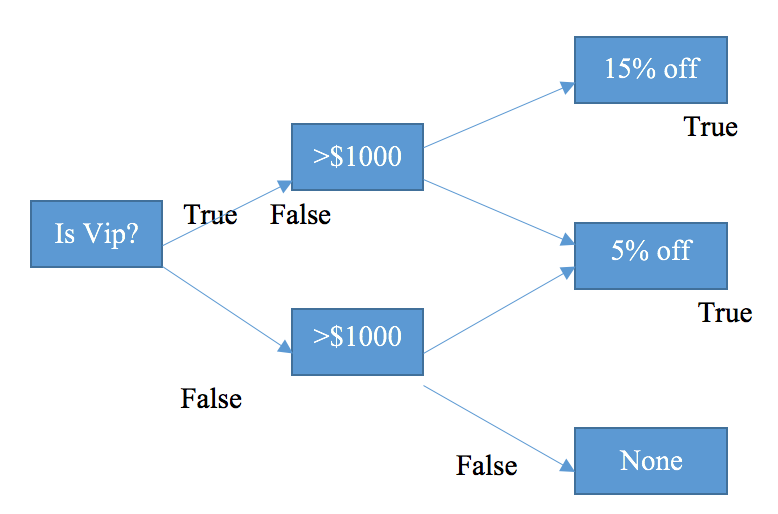
\includegraphics[width=8.0cm]{ctree.png} 
\newline
\caption{An Example of C4.
5 Decision Tree}
\label{fig:ctree} 
\end{figure}

We adopt C4.
5 to generate a decision tree for the problem.
 The algorithm is proposed by Ross Quinlan~\cite{quinlan}, which is an extension of his earlier ID3 algorithm.

The pseudocode~\cite{Kotsiantis} of the general algorithm for building decision trees by C4.
5 is: 

\begin{enumerate}
\item Check for base cases.

\item For each attribute a, find the normalized information gain ratio from splitting on a.

\item Let a\_best be the attribute with the highest normalized information gain.

\item Create a decision node that splits on a\_best.

\item Recur on the sublists obtained by splitting on a\_best, and add those nodes as the children of the node.

\end{enumerate}



\section{Experiments}
In this section, we will introduce the data collection, data sets, and how we conduct the experiments.
\subsection{Data Collection}
All the data comes from Dotabuff, which is the largest third-party Dota2 game track website.
In the team section of Dotabuff, there are more than 1,000 teams sharing their game results.
We write a crawler to collect the game data by Python urllib2 and Beautifulsoup libraries.
As Section IV mentioned, from each game, we can get the 111 hero usage, 30 synergic pairs of heroes usage,
30 conter pairs of heroes usage, game running time, and the final result.
We kept running the crawler for four days to collect data.
\subsection{Data Sets}
Our data sets include 15,197 Dota2 matches records from top 100 win-rate teams in the world.
Each feature vector includes 111 hero feature, 30 synergic pair feature, 30 conter pair feature,
1 game time feature, and 1 game result feature.
In total, there are 173 features in the feature vector.

\subsection{Training and Testing}
We use 10-fold cross-validation as our training and testing methods.
The original data sets are randomly partitioned into 10 equal sized subsets, use one of the subsets as the test set and the others as the testing set.
The process is to repeate 10 folds, with each subset used exactly once as the testing set.
The results are the combined from 10 folds.

\subsection{Evaluation Metrics}
Evaluation of performance of a classification model is decided by the number of correctly classified instances and incorrectly classified instances. These counts are tabulated into a table called confusion matrix. In addition to this, performance metrics are used for comparing performances between different models, for example, accuracy and error rate:

\begin{equation}
Accuracy = \frac{Number\ of\ correct\ predictions}{Total\ number\ of\ predictions}
\end{equation}

\begin{equation}
Error\ rate = \frac{Number\ of\ wrong\ predictions}{Total\ number\ of\ predictions}
\end{equation}

F-score is used as the evaluation metric our experiment, since both the precision and recall are considered by this method.
F-score can be calculated by the following formulas.

\begin{equation}
F=2\times\frac{Precision+Recall}{Precision*Recall}
\end{equation}

\begin{equation}
Precision = \frac{TruePositives}{TruePositives+FalsePositives}
\end{equation}

\begin{equation}
Recall = \frac{TruePositives}{TruePositives+FalseNegatives}
\end{equation}

We also use Confusion Matrix to present our results.
A sample form is described in Table~\ref{table:sample}.
There are 200 samples in the testing data set.
200 instances are classified correctly, and 100 instances are classified wrongly.

\begin{table}
\begin{center}
\begin{tabular}{|c|c|c|}
\hline
Predicted: True & Predicted: False & N = 200 \\ \hline
100 & 50 & Actual: True \\ \hline
50 & 100 & Actual: False \\ \hline
\end{tabular}
\caption{A Sample of Confusion Matrix}
\label{table:sample}
\end{center}
\end{table}

\subsection{Decision Tree}
In this given dataset, we adopt decision tree with 10-fold cross-validation for this problem. Correctly Classified Instances are 8576 which takes 58.0479 \%. And Incorrectly Classified Instances are 6198 which takes 41.9521 \%. The accuracy by class and confusion matrix can be seen in Table~\ref{table:dtreeaccuracy} and Table~\ref{table:dtreeconfusionmatrix}.

\begin{table}
\begin{center}
\begin{tabular}{|c|c|c|c|}
\hline
Class & Precision & Recall & F-score \\ \hline
win & 0.853 & 0.162 & 0.272 \\ \hline
lose & 0.553 & 0.974 & 0.705 \\ \hline
\end{tabular}
\caption{Detailed Accuracy by Class}
\label{table:dtreeaccuracy}
\end{center}
\end{table}

\begin{table}
\begin{center}
\begin{tabular}{|c|c|c|}
\hline
a & b & \\ \hline
1158 & 5999 & a = win \\ \hline
199 & 7418 & b = lose \\ \hline
\end{tabular}
\caption{Confusion Matrix of Decision Tree}
\label{table:dtreeconfusionmatrix}
\end{center}
\end{table}


Usually, there is a tradeoff between precision and recall. The higher precision, the lower recall or the lower precision, the higher recall. From the result, we know that in win class, it has high precision but low recall and in lose class, it has low precision and high recall. That's because lots of win instances are misclassified into lose. The false positive is large.

\subsection{SVM}

The following figure shows the result of SVM. When the value of C increases, the accuracy rate increase from 51.65\% to 58.55\%. After the point, the accuracy rate won't increase much. We found that the radial basis kernel works better than linear kernel for this problem. (Accuarcy rate of 58.55\% compares with 57.9\%) After analyzing data, we thinks this is because our data are not linear-separable. Applying radial basis function, the original feature space is mapped to another feature space with high dimension. In the new feature space, these data are linear-separable. In addition, kernel trick makes sure that the calculation in high dimension won’t cost too much time.

\begin{figure}[!htbp]
\centering
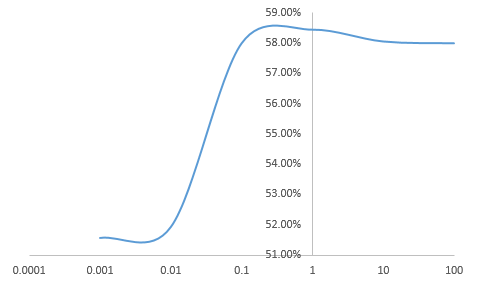
\includegraphics[width=8.0cm]{svmcurve.PNG} 
\newline
\caption{Result of SVM with Different C}
\label{fig:svmcurve} 
\end{figure}


We adopt support vector machine with 10-fold cross-validation for this problem. Correctly Classified Instances are 9445 which takes 58.5528 \%. And Incorrectly Classified Instances are 6694 which takes 41.4772 \%. 


\subsection{Results from Other Models}
We also applied other models to the problem.
 The results are shown in Table~\ref{table:others}

\begin{table}
\begin{center}
\begin{tabular}{|c|c|}
\hline
Model & Accuracy Rate \\ \hline
Decision Tree & 58.05\% \\ \hline
Natural Network & 54.98\% \\ \hline
Support Vector Machine & 58.55\% \\ \hline
Naive Bayes & 56.07\% \\ \hline
Adaboost & 55.35\% \\ \hline
\end{tabular}
\caption{Results from Other Models}
\label{table:others}
\end{center}
\end{table}

In adaboost method, we used decision tree as a classifier of it. However, we didn't find an obvious relationship between accuracy rate and the number of weak classifiers. We believe the result could be improved with more testing.

\subsection{K-nearest neighbor}

We adopt K-nearest neighbor as we discussed in the design part. After training the synergic-counter pairs, we get the final result. Correctly Classified Instances are 8576 which takes 75.1038 \%. And Incorrectly Classified Instances are 6198 which takes 24.8962 \%. The accuracy by class and confusion matrix can be seen in Table~\ref{table:knnaccuracy} and Table~\ref{table:knnconfusionmatrix}.

\begin{table}
\begin{center}
\begin{tabular}{|c|c|c|c|}
\hline
Class & Precision & Recall & F-score \\ \hline
win & 0.702 & 0.770 & 0.734 \\ \hline
lose & 0.799 & 0.736 & 0.766 \\ \hline
\end{tabular}
\caption{Detailed Accuracy by Class}
\label{table:knnaccuracy}
\end{center}
\end{table}

\begin{table}
\begin{center}
\begin{tabular}{|c|c|c|}
\hline
a & b & \\ \hline
5546 & 1659 & a = win \\ \hline
2359 & 6575 & b = lose \\ \hline
\end{tabular}
\caption{Confusion Matrix of Decision Tree}
\label{table:knnconfusionmatrix}
\end{center}
\end{table}

From this result, we know that this modified method largely improved accuracy rate.

\subsection{Comparison with Other Exisiting Algorithms}

\begin{table}
\centering
\begin{tabular}{|c|c|}
\hline
Algorithm & Accuracy \\ \hline
Our algorithm & 75.1\% \\ \hline 
Kalyanaraman's & 74.1\% \\ \hline
Conley's & 69.8\% \\ \hline
\end{tabular}
\caption{Performance Comparison}
\label{table:comp}
\end{table}

In this subseciton, we simply show the performance comparion between our algorithm and other exisiting algorithms.
The details can be seen in Table~\ref{table:comp}



\section{Related Work}
Conley et al.~\cite{conley2013does} did a research on which machine learning method is the best for data game results.
However, they only focus on two machine learning approaches, linear regression and k-nearest neighbour(kNN).
In our paper, we focus on four mainstream machine learning approaches.
Kalyannaraman~\cite{kau2013win} did an augmented algorithm on traditional linear regression considering pair relationships of heroes.
However, he did not consider all the relationship between heroes, like the restraint relationship between heroes.
In our research, we further consider the negative relationship of heroes and the time factor.
What's more, the data scale used in our research is much professional and larger than theirs.
It ensures that our research is more reliable and trusted.

Drachen et al. ~\cite{drachen2014skill} try to predict the temporal and spatial of players in the game based on the hero skills.
Semenov et al. ~\cite{semenovapplications} conclude the current research situation for Dota prediction
and show some opinoins of eSports game prediction.

\section{Conclusion}
This paper proposes a method to predict the eSports game results of Dota. Our lineup model for DotA2 matches represents an attempt to condense gameplay to the key part to analyze the match result. 
With three-type features (Team ID, Hero Lineup and Result) and decision tree model, our Dota prediction system gets 75.1\% accuracy rate from a data set of matches.
 
The accuracy rate is not relatively high and the reasons are as follows:
\begin{enumerate}
\item Concerning the data sets, we can only get the game records including the information of Team ID, Heroes Lineup and result.
More detailed information about teams and games are not available. For eample, a team with higher skills players and synergy among them would dominates in a match even if their opponent pick a superior lineup.

\item Regarding features, player’s styles and skills, physical and emotional condition and the external environment all are vital to the result of a game, but none of them can be measured.

\item DotA2 is a game of uncertainty with regards to the in-game mechanism. Many elements in the map are generated randomly or pseudo-randomly, such as type of runes, and Roshan respawn time. Other than that, many heroes skills are also random or pseudu-random coded.  Like poker games, luck can sometimes play an important role in E-Sports.

\end{enumerate}
Our results highlight that DotA is a game where many factors contributes to the matching result. In the future, we would like to include player's skill and style as part of the feature vector. An easier way is to assign weighted score to different E-sports teams. However, this approach's efficacy is narrowed because of team's fluidity and patch updates. Another way to improve the accuracy is to perform runtime analysis while game is playing and new data regarding the game information are retrieved. Both methods require scrutinizing and deep understanding the game mechanism.


\balance
\IEEEpeerreviewmaketitle

\bibliographystyle{abbrv}
\bibliography{./Template}

\end{document}
